% Drawing 74/03-9 -- folder 74, batch 03, archive page 53 (PDF page 54).
% Transcription: à gauche, un graphe : les sommets $p, q, r$ (en colonne) et $i, j, k$ (en colonne), joints par des traits pleins ($p$–$i$, $q$–$i$, $r$–$i$) et pointillés, avec une troisième colonne de points à droite reliés à $i$ par des pointillés.
% Kind: graph between two columns of vertices. Method 2 (schematic redraw from the facsimile). Status: ok.
% Notes: p, q, r in a column at the left and i, j, k in a second column; heavy strokes p-i, q-i and r-i, the last with an arrowhead at r; thin broken strokes from each of p, q, r to each of j and k (p-j, p-k, q-j, q-k, r-j, r-k), so that with the heavy strokes every one of the nine pairs is joined; at the right, a third column of three heavy points, each joined to i and to j: from i by broken strokes to the upper and middle points (the second ending in an arrowhead) and by a wavy stroke to the lower one, from j by broken strokes to the upper and middle points and by a thin stroke to the lower one. No points are drawn at p, q, r, i, j, k: there are none on the page. The label of the middle right vertex looks like « -k » and is given as j after the transcription; the marks lower down are separate. Overlay check 2026-11-13 (issue 147, Claude claude-opus-5-5): the redraw, rasterised by the skill's previewer (not compiled: no TeX in the session), laid over the 300 dpi colour crop of the scan (261 ppi). The earlier redraw lay 2 to 3 units off its ink, joined only p-k, q-k, r-j and r-k by thin strokes, and stopped at the bbox edge, which cut the third column: the bbox is widened to the right (from 0.30 to 0.34 of the page width), the coordinates rescaled to it, every stroke moved onto its ink, p-j and q-j added (each a broken stroke ending at the short dash before j), the third column and its six strokes drawn, and the vertex dots, which are not on the page, removed. Disagreement: the transcription joins the third column to i alone; on the page j is joined to it as well (docs/review/transcription-readings-128-2026-11-12.md, issue 145). Matches the facsimile.
% Coordinates: 1 unit = 1 mm = 1/100 of the crop width (bbox in page fractions: [0.05, 0.47, 0.34, 0.68]).
% Redrawn by Claude (claude-opus-5-5), issue #73, 2026-11-09; not checked by a human; not compiled (no TeX in the session).
% Checked by Claude (claude-opus-5-5) 2026-11-13 (issue #147): overlaid on the 300 dpi colour facsimile and corrected; not compiled (no TeX in the session). Status: ok.
% Rights: reproduces part of the work -- behind RENDER_TRANSCRIPTS, never published by itself.
\documentclass[tikz,border=3pt]{standalone}
\usepackage{amsmath,amssymb}
\usetikzlibrary{patterns,arrows.meta}
\tikzset{pencil/.style={black!45}, struck/.style={black!35}, mark/.style={circle,draw,inner sep=1.3pt}, pt/.style={circle,fill,inner sep=0.9pt}, opt/.style={circle,draw,fill=white,inner sep=1.1pt}}
\begin{document}
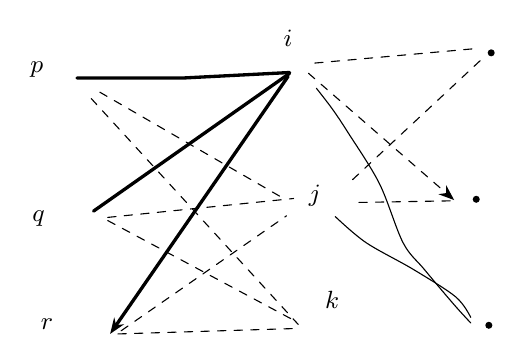
\begin{tikzpicture}[x=1mm,y=1mm,line cap=round,line join=round,font=\scriptsize]
\draw[very thick] (43.5,-16.6) -- (56.9,-16.6) -- (70.5,-15.9);
\draw[very thick] (70.5,-16) -- (45.6,-33.5);
\draw[very thick,-{Stealth[length=2mm]}] (70.3,-16.4) -- (47.7,-49.1);
\draw[dashed] (45.3,-19.2) -- (71.6,-47.9);
\draw[dashed] (46.4,-18.4) -- (69.4,-31.7);
\draw[dashed] (47.4,-34.3) -- (71,-31.9);
\draw[dashed] (47.4,-34.7) -- (71.1,-47.4);
\draw[dashed] (49.1,-48.7) -- (70.1,-34.1);
\draw[dashed] (48.7,-49.1) -- (71.6,-48.4);
\node[pt] at (96.1,-13.4) {};
\node[pt] at (94.2,-32) {};
\node[pt] at (95.8,-48) {};
\draw[dashed] (73.7,-14.7) -- (93.7,-12.9);
\draw[dashed,-{Stealth[length=2mm]}] (72.9,-16) -- (91.4,-32.1);
\draw plot[smooth, tension=0.55] coordinates {(73.9,-17.9) (75.9,-20.5) (77.9,-23.5) (81.9,-30) (84.9,-37.5) (87.6,-40.9) (91.4,-45.4) (93.5,-47.7)};
\draw[dashed] (78.5,-29.5) -- (94.8,-14.3);
\draw[dashed] (79.3,-32.4) -- (90.9,-32.2);
\draw plot[smooth, tension=0.55] coordinates {(76.3,-34.2) (80.2,-37.5) (86.2,-40.9) (91.6,-44.4) (93.5,-47)};
\node[inner sep=1pt] at (38.4,-15.5) {\small $p$};
\node[inner sep=1pt] at (38.6,-34.5) {\small $q$};
\node[inner sep=1pt] at (39.7,-47.8) {\small $r$};
\node[inner sep=1pt] at (70.3,-11.6) {\small $i$};
\node[inner sep=1pt] at (73.7,-31.5) {\small $j$};
\node[inner sep=1pt] at (75.9,-44.8) {\small $k$};
\end{tikzpicture}
\end{document}
